% !TEX program = xelatex
% 本科毕业设计答辩 Beamer 模板

\documentclass[aspectratio=169, 10pt]{beamer}

% ============================================================
% Packages
% ============================================================
\usepackage[UTF8, fontset=fandol]{ctex}
\usepackage{amsmath, amssymb, bm}
\usepackage{graphicx}
\usepackage{booktabs}
\usepackage{tabularx}
\usepackage{array}
\usepackage{multirow}
\usepackage{colortbl}
\usepackage{xcolor}
\usepackage{tikz}
\usetikzlibrary{arrows.meta, positioning, calc, shapes.geometric}
\usepackage{hyperref}

% 图片路径：按需修改
\graphicspath{
    {./figures/}
}

% ============================================================
% 视觉系统：Madrid + 浙大蓝
% ============================================================
\usetheme{Madrid}
\usecolortheme{default}

\definecolor{ZJUBlue}{RGB}{0, 75, 122}
\definecolor{ZJULight}{RGB}{70, 130, 180}
\definecolor{ZJUGold}{RGB}{196, 160, 52}
\definecolor{ZJUGray}{RGB}{107, 114, 128}
\definecolor{ZJUGreen}{RGB}{46, 125, 50}
\definecolor{ZJURed}{RGB}{198, 40, 40}
\definecolor{SoftGray}{RGB}{248, 251, 253}
\definecolor{LineGray}{RGB}{208, 215, 222}
\definecolor{CodeBg}{RGB}{248, 250, 252}
\definecolor{TitleBlue}{RGB}{234, 244, 250}
\definecolor{SOTAPink}{RGB}{252, 232, 237}

\setbeamercolor{palette primary}{bg=ZJUBlue, fg=white}
\setbeamercolor{palette secondary}{bg=ZJULight, fg=white}
\setbeamercolor{palette tertiary}{bg=ZJUBlue, fg=white}
\setbeamercolor{structure}{fg=ZJUBlue}
\setbeamercolor{title}{fg=white, bg=ZJUBlue}
\setbeamercolor{frametitle}{fg=ZJUBlue, bg=TitleBlue}
\setbeamercolor{block title}{bg=TitleBlue, fg=ZJUBlue}
\setbeamercolor{block body}{bg=ZJUBlue!5, fg=black}
\setbeamercolor{block title alerted}{bg=ZJURed!12, fg=ZJURed!85!black}
\setbeamercolor{block body alerted}{bg=ZJURed!5, fg=black}
\setbeamercolor{block title example}{bg=ZJUGreen!13, fg=ZJUGreen!70!black}
\setbeamercolor{block body example}{bg=ZJUGreen!4, fg=black}
\setbeamercolor{item}{fg=ZJUBlue}
\setbeamertemplate{blocks}[rounded][shadow=false]
\setbeamertemplate{itemize item}{\raise0.15ex\hbox{\scriptsize$\bullet$}}
\setbeamertemplate{itemize subitem}{\raise0.15ex\hbox{\tiny$\bullet$}}

\setbeamerfont{title}{size=\Large, series=\bfseries}
\setbeamerfont{subtitle}{size=\normalsize}
\setbeamerfont{frametitle}{size=\large, series=\bfseries}
\setbeamerfont{framesubtitle}{size=\small}
\setbeamertemplate{navigation symbols}{}
\setbeamertemplate{headline}{}
\setbeamertemplate{frametitle}{%
  \nointerlineskip
  \begin{beamercolorbox}[wd=\paperwidth,ht=0.70cm,dp=0.18cm]{frametitle}
    \hbox to \paperwidth{%
      \hspace*{0.55cm}%
      \vbox to 0.70cm{\vfil\hbox{\large\bfseries\insertframetitle}\vfil}%
      \hfil\hspace*{0.55cm}%
    }%
  \end{beamercolorbox}
  \vspace{0.05cm}
}
\definecolor{FootGray}{RGB}{156,163,175}
\setbeamertemplate{footline}{%
  \leavevmode%
  \vbox{%
    \hbox{\hspace*{0.45cm}\color{LineGray}\rule{\dimexpr\paperwidth-0.90cm\relax}{0.3pt}}%
    \hbox{%
      \begin{beamercolorbox}[wd=.28\paperwidth,ht=2.8ex,dp=1.0ex,leftskip=0.45cm]{normal text}%
        {\fontsize{7.5}{9}\selectfont\color{FootGray}答辩人姓名 | XXXXXXXXXX}%
      \end{beamercolorbox}%
      \begin{beamercolorbox}[wd=.52\paperwidth,ht=2.8ex,dp=1.0ex,center]{normal text}%
        {\fontsize{7.5}{9}\selectfont\color{FootGray}论文中文标题}%
      \end{beamercolorbox}%
      \begin{beamercolorbox}[wd=.20\paperwidth,ht=2.8ex,dp=1.0ex,rightskip=0.45cm plus1fil]{normal text}%
        {\fontsize{7.5}{9}\selectfont\color{FootGray}\insertframenumber/\inserttotalframenumber}%
      \end{beamercolorbox}%
    }%
  }%
}

% ============================================================
% Helpers
% ============================================================
\newcommand{\slidekey}[1]{}

\newcommand{\sectioncover}[3]{%
  {
  \setbeamertemplate{footline}{}
  \begin{frame}[plain]
    \begin{tikzpicture}[remember picture,overlay]
      \fill[white] (current page.south west) rectangle (current page.north east);
      \fill[TitleBlue] (current page.north west) rectangle ([yshift=-0.78cm]current page.north east);
      \draw[LineGray,line width=0.4pt]
        ([xshift=0.75cm,yshift=-0.78cm]current page.north west) --
        ([xshift=-0.75cm,yshift=-0.78cm]current page.north east);
      \node[anchor=north east, xshift=-0.72cm, yshift=-0.18cm] at (current page.north east)
        {\includegraphics[height=0.58cm]{zjuchar.pdf}};
      \node[anchor=west, text=ZJUBlue, font=\Large\bfseries] at ([xshift=1.25cm,yshift=-2.35cm]current page.north west) {#1};
      \node[
        anchor=west,
        text=ZJUBlue,
        font=\fontsize{24}{29}\selectfont\bfseries,
        text width=8.3cm,
        align=left
      ] at ([xshift=1.25cm,yshift=-3.18cm]current page.north west) {#2};
      \node[
        anchor=west,
        text=ZJUGray,
        font=\normalsize,
        text width=9.2cm,
        align=left
      ] at ([xshift=1.25cm,yshift=-4.10cm]current page.north west) {#3};
      \draw[LineGray,line width=0.75pt]
        ([xshift=1.25cm,yshift=-4.88cm]current page.north west) --
        ([xshift=8.20cm,yshift=-4.88cm]current page.north west);
    \end{tikzpicture}
  \end{frame}
  }
}

\newcommand{\tagbox}[2][ZJUBlue]{%
  \tikz[baseline=(n.base)]\node[
    fill=#1!9,
    draw=#1!55,
    rounded corners=2pt,
    inner xsep=4pt,
    inner ysep=2pt
  ] (n) {\scriptsize\bfseries\textcolor{#1}{#2}};
}

\newcommand{\metric}[3]{%
  \begin{tikzpicture}
    \node[
      fill=SoftGray,
      draw=LineGray,
      rounded corners=3pt,
      minimum width=3.0cm,
      minimum height=1.05cm,
      align=center
    ] {
      {\scriptsize #1}\\[-1pt]
      {\Large\bfseries\textcolor{ZJUBlue}{#2}}\\[-1pt]
      {\scriptsize\textcolor{ZJUGreen}{#3}}
    };
  \end{tikzpicture}
}

\newenvironment{compactitem}{%
  \begin{itemize}
    \setlength{\itemsep}{3pt}
    \setlength{\parskip}{0pt}
    \setlength{\parsep}{0pt}
}{\end{itemize}}

\newenvironment{compactenum}{%
  \begin{enumerate}
    \setlength{\itemsep}{4pt}
    \setlength{\parskip}{0pt}
    \setlength{\parsep}{0pt}
}{\end{enumerate}}

\newcolumntype{Y}{>{\raggedright\arraybackslash}X}
\newcommand{\smalltab}{\scriptsize\renewcommand{\arraystretch}{1.16}}

\tikzset{
  module/.style={
    fill=#1!12,
    draw=#1!50,
    rounded corners=3pt,
    minimum height=0.72cm,
    align=center,
    inner sep=4pt,
    font=\scriptsize
  },
  flow/.style={
    -{Stealth[length=4pt,width=3.5pt]},
    thick,
    color=ZJUBlue!70
  }
}

% ============================================================
% Metadata — 按需填写个人信息
% ============================================================
\title[论文简称]{论文中文标题\\论文中文副标题}
\subtitle{本科毕业论文答辩}
\author[答辩人姓名]{答辩人：答辩人姓名；学号：XXXXXXXXXX；指导教师：XXX老师}
\institute[XX大学]{XX学院 \quad 20XX 级XX专业}
\date{20XX 年 X 月 X 日}

\begin{document}

% ==================== Cover ====================
{
\setbeamertemplate{footline}{}
\setbeamertemplate{frametitle}{}
\begin{frame}[plain]
  \begin{tikzpicture}[remember picture,overlay]
    \fill[white] (current page.south west) rectangle (current page.north east);
    \fill[TitleBlue] (current page.north west) rectangle ([yshift=-0.82cm]current page.north east);
    \draw[LineGray,line width=0.4pt]
      ([xshift=0.65cm,yshift=-0.82cm]current page.north west) --
      ([xshift=-0.65cm,yshift=-0.82cm]current page.north east);
    \node[anchor=north west, text=ZJUBlue, font=\bfseries\normalsize]
      at ([xshift=0.78cm,yshift=-0.23cm]current page.north west) {本科毕业论文答辩};
    \node[anchor=north east, xshift=-0.72cm, yshift=-0.16cm] at (current page.north east)
      {\includegraphics[height=0.58cm]{zjuchar.pdf}};
    \node[anchor=north west, text=ZJUBlue, font=\fontsize{20}{25}\selectfont\bfseries]
      at ([xshift=0.95cm,yshift=-1.78cm]current page.north west) {论文中文标题};
    \node[anchor=north west, text=ZJUBlue, font=\fontsize{20}{25}\selectfont\bfseries]
      at ([xshift=0.95cm,yshift=-2.55cm]current page.north west) {论文中文副标题};
    \node[
      anchor=north west,
      text=ZJUGray,
      font=\fontsize{9}{11}\selectfont,
      text width=14.5cm,
      align=left
    ] at ([xshift=0.95cm,yshift=-3.42cm]current page.north west)
      {English Title of the Thesis};
    \draw[LineGray,line width=0.7pt]
      ([xshift=0.95cm,yshift=-4.52cm]current page.north west) --
      ([xshift=10.90cm,yshift=-4.52cm]current page.north west);
    \node[anchor=north, font=\normalsize, align=center]
      at ([yshift=-5.02cm]current page.north) {%
        \renewcommand{\arraystretch}{1.28}
        \begin{tabular}{r@{\quad}l}
          \textcolor{ZJUGray}{答辩人} & \textbf{答辩人姓名} \\
          \textcolor{ZJUGray}{学号} & \textbf{XXXXXXXXXX} \\
          \textcolor{ZJUGray}{指导教师} & \textbf{XXX老师} \\
          \textcolor{ZJUGray}{学院} & \textbf{XX学院} \\
          \textcolor{ZJUGray}{专业} & \textbf{20XX 级XX专业} \\
          \textcolor{ZJUGray}{日期} & \textbf{20XX 年 X 月 X 日}
        \end{tabular}
      };
  \end{tikzpicture}
\end{frame}
}

% ==================== Outline ====================
\begin{frame}{目录}
  \vspace{0.28cm}
  \centering
  \begin{tikzpicture}[x=1cm,y=1cm]
    \node[fill=TitleBlue,draw=ZJUBlue!28,rounded corners=3pt,minimum width=6.25cm,minimum height=1.34cm,align=left,text width=5.55cm,inner xsep=0.35cm]
      at (-3.45,0) {\textbf{\textcolor{ZJUBlue}{01 研究背景与动机}}\\[2pt]\scriptsize 研究背景简介};
    \node[fill=TitleBlue,draw=ZJUBlue!28,rounded corners=3pt,minimum width=6.25cm,minimum height=1.34cm,align=left,text width=5.55cm,inner xsep=0.35cm]
      at (3.45,0) {\textbf{\textcolor{ZJUBlue}{03 实验验证}}\\[2pt]\scriptsize 实验设置与结果分析};
    \node[fill=TitleBlue,draw=ZJUBlue!28,rounded corners=3pt,minimum width=6.25cm,minimum height=1.34cm,align=left,text width=5.55cm,inner xsep=0.35cm]
      at (-3.45,-1.72) {\textbf{\textcolor{ZJUBlue}{02 方法设计}}\\[2pt]\scriptsize 方法概述与关键模块};
    \node[fill=TitleBlue,draw=ZJUBlue!28,rounded corners=3pt,minimum width=6.25cm,minimum height=1.34cm,align=left,text width=5.55cm,inner xsep=0.35cm]
      at (3.45,-1.72) {\textbf{\textcolor{ZJUBlue}{04 总结与展望}}\\[2pt]\scriptsize 贡献与未来方向};
  \end{tikzpicture}
\end{frame}

% ============================================================
\section{研究背景与动机}
% ============================================================
\sectioncover{01}{研究背景与动机}{}

\begin{frame}{视频生成模型与物理常识挑战}
  \slidekey{新一代视频生成模型已经能生成较高质量的开放域视频，但物理常识仍是高频短板。}

  \begin{block}{新一代世界模型（视频生成模型）}
    \begin{compactitem}
      \item Sora、Veo、Kling、Wan 等模型已能根据文本提示生成高分辨率的视频，初步具备对真实世界的建模能力。
      \item 支持文本到视频、图像到视频等多种生成模式，单帧画质和时间一致性持续提升。
      \item 该方向正在从单纯的内容生成向世界模拟器演进，有望成为机器人仿真、具身智能和科学可视化的基础工具。
    \end{compactitem}
  \end{block}

  \vspace{0.30cm}
  \begin{alertblock}{物理常识缺陷}
    \begin{compactitem}
      \item \textbf{现状：}物体穿透、重力失效、碰撞无响应，材料形变与流体边界失真等。
      \item \textbf{表现：}模型倾向于生成视觉上"好看"但不符合物理规律的视频。
      \item \textbf{为何重要：}缺乏物理常识的视频模型无法支撑需要物理一致性的下游任务，如机器人策略学习和自动驾驶仿真。
    \end{compactitem}
  \end{alertblock}

\end{frame}

\begin{frame}{现有方案的困境}
  \slidekey{显式仿真、统一大模型、离线偏好优化各有代价；在线 VLM 反馈可作为轻量后训练信号。}

  \begin{columns}[T,onlytextwidth]
    \begin{column}{0.31\textwidth}
      \begin{block}{\centering 显式物理引擎}
        \small
        \textcolor{ZJUGreen!70!black}{\textbf{优势：}}封闭场景中物理约束明确，可解释性强。

        \vspace{0.08cm}
        \textcolor{ZJURed}{\textbf{困境：}}开放域场景远超仿真器覆盖范围，需要精确初始条件，文本提示通常无法提供。
      \end{block}
    \end{column}%
    \begin{column}{0.31\textwidth}
      \begin{block}{\centering 统一多模态大模型}
        \small
        \textcolor{ZJUGreen!70!black}{\textbf{优势：}}从头预训练融合理解与生成，能力完整。

        \vspace{0.08cm}
        \textcolor{ZJURed}{\textbf{困境：}}需数千 GPU 和 PB 级数据，物理正确视频占比极小，易拟合虚假统计模式。
      \end{block}
    \end{column}%
    \begin{column}{0.31\textwidth}
      \begin{block}{\centering 离线对齐}
        \small
        \textcolor{ZJUGreen!70!black}{\textbf{优势：}}不需要在线采样，从配对好坏视频数据中学习偏好。

        \vspace{0.08cm}
        \textcolor{ZJURed}{\textbf{困境：}}训练数据固定，模型无法探索新策略并获得即时反馈，静态偏好数据无法持续改进。
      \end{block}
    \end{column}
  \end{columns}

  \vspace{0.18cm}
  \begin{tikzpicture}
    \node[
      fill=TitleBlue,
      draw=ZJUBlue!35,
      rounded corners=4pt,
      text width=0.96\textwidth,
      align=center,
      inner sep=0.18cm
    ] {\small\textbf{\textcolor{ZJUBlue}{研究动机}}\\[2pt]在不依赖物理模拟器的前提下，通过视觉语言模型反馈和在线强化学习\\让世界模型生成的视频更符合物理规律。};
  \end{tikzpicture}
\end{frame}

\begin{frame}{主要工作与贡献}
  \slidekey{围绕"数据、奖励、算法、验证"四个环节构建完整后训练闭环。}

  \vspace{0.12cm}
  \begin{columns}[T,onlytextwidth]
    \begin{column}{0.48\textwidth}
      \begin{block}{1. 构建物理提示词集}
        \small 构建并筛选物理提示词数据集，覆盖重力碰撞、材料流体等方面。
      \end{block}
      \begin{block}{2. 视觉语言模型双维度奖励}
        \small 通过 PC 和 SA 两个维度，分别约束物理常识和语义贴合，减少奖励作弊行为。
      \end{block}
    \end{column}%
    \begin{column}{0.48\textwidth}
      \begin{block}{3. 强化学习后训练策略}
        \small 参照 Flow-GRPO 论文实现代码，完成 SDE 采样、群组相对优势估计与 LoRA 参数更新。
      \end{block}
      \begin{block}{4. 多维度实验验证}
        \small 通过 VBench2.0、人工偏好、消融实验和跨模型实验验证训练有效性。
      \end{block}
    \end{column}
  \end{columns}
\end{frame}

% ============================================================
\section{方法设计}
% ============================================================
\sectioncover{02}{方法设计}{}

% ====== 方法设计：提示词构建 ======

\begin{frame}{物理事件提示词构建}
  \slidekey{提示词构建是方法的一部分：把普通场景描述转化为可生成、可观察、可评价的物理事件。}

  \centering
  \includegraphics[width=0.88\paperwidth,height=0.55\paperheight,keepaspectratio]{prompt_dataset_pipeline.pdf}
\end{frame}

\begin{frame}{提示词构建：三阶段流程与设计原则}
  \slidekey{三阶段流程保证提示词质量，设计原则确保奖励聚焦物理事件。}

  \begin{columns}[T,onlytextwidth]
    \begin{column}{0.48\textwidth}
      \begin{block}{三阶段流程}
        \begin{compactenum}
          \item \textbf{候选生成：}围绕物理常识，由大语言模型批量构造描述。
          \item \textbf{物理筛选：}由 GPT-4o 判断候选是否真正涉及物理事件，剔除静态场景。
          \item \textbf{人工筛查：}处理边界样本与歧义结果，保证最终提示词可观察、可评价。
        \end{compactenum}
      \end{block}
    \end{column}%
    \begin{column}{0.48\textwidth}
      \begin{exampleblock}{设计原则}
        \begin{compactitem}
          \item \textbf{明确三要素：}每条提示词必须包含初始状态、动作过程和可观察后果。
          \item \textbf{排除不可评样本：}排除静态氛围、隐藏状态和多义结果。
          \item \textbf{聚焦物理事件：}让奖励聚焦物理事件本身，而非一般视觉质量。
        \end{compactitem}
      \end{exampleblock}

    \end{column}
  \end{columns}
\end{frame}

\begin{frame}{提示词生成与筛选模板}
  \slidekey{生成模板关注"初始状态、动作过程、可观察后果"，筛选模板剔除静态、不可评价或结果歧义样本。}

  \begin{columns}[T,onlytextwidth]
    \begin{column}{0.48\textwidth}
      \textbf{\textcolor{ZJUBlue}{生成候选提示词的模板}}
      \vspace{0.10cm}

      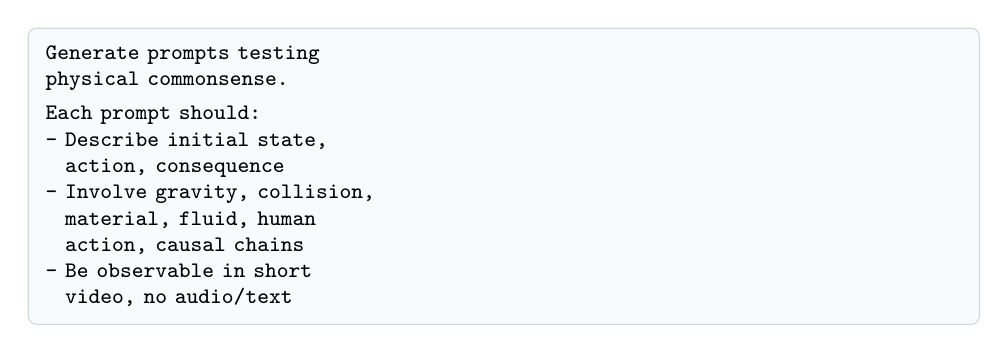
\begin{tikzpicture}
        \node[
          fill=CodeBg,
          draw=LineGray,
          rounded corners=3pt,
          text width=0.96\textwidth,
          align=left,
          inner sep=0.22cm,
          font=\footnotesize\ttfamily
        ] {
          Generate prompts testing\\
          physical commonsense.\\[3pt]
          Each prompt should:\\
          - Describe initial state,\\
          \phantom{- }action, consequence\\
          - Involve gravity, collision,\\
          \phantom{- }material, fluid, human\\
          \phantom{- }action, causal chains\\
          - Be observable in short\\
          \phantom{- }video, no audio/text
        };
      \end{tikzpicture}
    \end{column}%
    \begin{column}{0.48\textwidth}
      \textbf{\textcolor{ZJUBlue}{GPT-4o 筛选的提示词}}
      \vspace{0.10cm}

      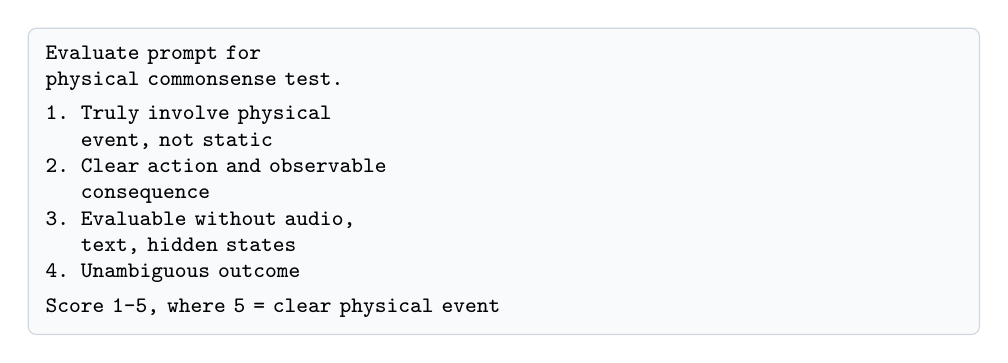
\begin{tikzpicture}
        \node[
          fill=CodeBg,
          draw=LineGray,
          rounded corners=3pt,
          text width=0.96\textwidth,
          align=left,
          inner sep=0.22cm,
          font=\footnotesize\ttfamily
        ] {
          Evaluate prompt for\\
          physical commonsense test.\\[3pt]
          1. Truly involve physical\\
          \phantom{1. }event, not static\\
          2. Clear action and observable\\
          \phantom{2. }consequence\\
          3. Evaluable without audio,\\
          \phantom{3. }text, hidden states\\
          4. Unambiguous outcome\\[3pt]
          Score 1-5, where 5 = clear physical event
        };
      \end{tikzpicture}
    \end{column}
  \end{columns}
\end{frame}

% ====== 方法设计：后训练策略 ======

\begin{frame}{强化学习后训练策略总览}
  \slidekey{系统采用 Actor-VLM Judge-Trainer 架构：在线生成候选视频，视觉语言模型打分，强化学习更新 LoRA 参数。}

  \centering
  \includegraphics[width=0.90\paperwidth,height=0.59\paperheight,keepaspectratio]{vlm_feedback_physical_alignment.pdf}
\end{frame}

\begin{frame}{视觉语言模型双维度奖励}
  \slidekey{PC 奖励约束物理常识，SA 奖励约束语义完成度，两者共同减少奖励作弊。}

  \begin{columns}[T,onlytextwidth]
    \begin{column}{0.48\textwidth}
      \begin{block}{物理常识奖励 PC}
        \begin{compactitem}
          \item 重力方向与运动趋势是否合理。
          \item 碰撞响应、不可穿透约束。
          \item 材料形变、液体边界。
        \end{compactitem}
        \vspace{0.08cm}
        \centering \tagbox[ZJURed]{$r_{\mathrm{PC}}$}
      \end{block}
      \vspace{0.10cm}
      
\begin{tikzpicture}
        \node[
          fill=CodeBg,
          draw=LineGray,
          rounded corners=3pt,
          text width=0.95\textwidth,
          align=left,
          inner sep=0.14cm,
          font=\scriptsize\ttfamily
        ] {
          Role: Expert in physical commonsense.\\
          Criteria: motion, force, gravity, collisions,\\
          \phantom{Criteria: }material, causality.\\
          Output: Score: X (1-5)
        };
      \end{tikzpicture}
    \end{column}%
    \begin{column}{0.48\textwidth}
      \begin{exampleblock}{语义贴合奖励 SA}
        \begin{compactitem}
          \item 主体、动作、场景是否出现。
          \item 关键视觉细节是否匹配。
          \item 防止静止化或模糊化逃避物理错误。
        \end{compactitem}
        \vspace{0.08cm}
        \centering \tagbox[ZJUGreen]{$r_{\mathrm{SA}}$}
      \end{exampleblock}
      \vspace{0.10cm}
      
\begin{tikzpicture}
        \node[
          fill=CodeBg,
          draw=LineGray,
          rounded corners=3pt,
          text width=0.95\textwidth,
          align=left,
          inner sep=0.14cm,
          font=\scriptsize\ttfamily
        ] {
          Role: Expert video analysis judge.\\
          Criteria: objects, actions, scene,\\
          \phantom{Criteria: }temporal order, visual details.\\
          Output: Score: X (1-5)
        };
      \end{tikzpicture}
    \end{column}
  \end{columns}

\end{frame}

\begin{frame}{强化学习后训练策略优化}
  \slidekey{核心思想：用 VLM 奖励信号指导视频生成模型，通过截断策略梯度和 KL 正则化稳定训练。}

  \begin{block}{Flow-GRPO 的损失函数}
    \small
    \[
    L = \underbrace{-\mathbb{E}\!\left[\min\!\left(\rho_t\,\hat A,\,
    \operatorname{clip}(\rho_t,1\!-\!\varepsilon,1\!+\!\varepsilon)\,\hat A\right)\right]}_{L_{\mathrm{pg}}\text{：策略梯度损失}}
    \;+\;
    \underbrace{\beta \cdot L_{\mathrm{KL}}}_{\text{KL 正则项}}
    \]
  \end{block}

  \begin{columns}[T,onlytextwidth]
    \begin{column}{0.32\textwidth}
      \begin{exampleblock}{策略比值 $\rho_t$}
        \begin{minipage}[t][3.0cm]{\textwidth}
          \scriptsize
          \[
          \rho_t=\frac{p_\theta(z_{t-1}|z_t,c)}
          {p_{\theta_{\mathrm{old}}}(z_{t-1}|z_t,c)}
          \]
          {\normalfont 衡量新旧策略在同一转移上的概率比。$\rho_t>1$ 表示新策略更倾向于该动作。}
          \vfill
        \end{minipage}
      \end{exampleblock}
    \end{column}%
    \begin{column}{0.32\textwidth}
      \begin{exampleblock}{优势估计 $\hat A$}
        \begin{minipage}[t][3.0cm]{\textwidth}
          \scriptsize
          \[
          \hat A=w_{\mathrm{PC}}\hat A_{\mathrm{PC}}+
          w_{\mathrm{SA}}\hat A_{\mathrm{SA}}
          \]
          {\normalfont 群组内标准化后的奖励，$\hat A>0$ 表示优于平均水平。}\\[2pt]
          \[
          \hat A_h=\frac{r_h-\mu_{c,h}}{\sigma_{c,h}+\epsilon}
          \]
          \vfill
        \end{minipage}
      \end{exampleblock}
    \end{column}%
    \begin{column}{0.32\textwidth}
      \begin{exampleblock}{KL 正则项 $L_{\mathrm{KL}}$}
        \begin{minipage}[t][3.0cm]{\textwidth}
          \scriptsize
          \[
          L_{\mathrm{KL}}=\frac{\|\mu_\theta-\mu_{\mathrm{ref}}\|_2^2}{2\sigma_t^2\Delta t}
          \]
          {\normalfont 约束当前策略不偏离参考模型太远，防止灾难性遗忘。}
          \vfill
        \end{minipage}
      \end{exampleblock}
    \end{column}
  \end{columns}

  \vspace{0.06cm}
  \begin{tikzpicture}
    \node[
      fill=TitleBlue,
      draw=ZJUBlue!35,
      rounded corners=3pt,
      text width=0.96\textwidth,
      align=left,
      inner sep=0.14cm,
      font=\scriptsize
    ] {\textbf{直觉理解：}$\rho_t\hat A>0$ 时增大该转移概率，$\rho_t\hat A<0$ 时减小；clip 限制单步更新幅度，$\beta$ 控制保守程度。};
  \end{tikzpicture}
\end{frame}

\begin{frame}{代码实现流程}
  \slidekey{基于视觉语言模型评估的强化学习后训练策略的代码实现流程。}

  \small
  \textbf{输入：}基础生成器 $\pi_{\theta_0}$，参考策略 $\pi_{\mathrm{ref}}$，提示词集 $\mathcal{D}$，评估器 $J_{\mathrm{PC}}$ 和 $J_{\mathrm{SA}}$，组大小 $G$，KL 权重 $\beta$，截断范围 $\varepsilon$

  \vspace{0.12cm}
  \begin{tikzpicture}
    \node[
      fill=CodeBg,
      draw=LineGray,
      rounded corners=4pt,
      text width=0.96\textwidth,
      align=left,
      inner sep=0.20cm,
      font=\footnotesize
    ] {
      \begin{minipage}{\dimexpr\textwidth-0.44cm}
        \begin{tabbing}
        \hspace{1.6em}\= \hspace{1.6em}\= \hspace{1.6em}\= \hspace{1.6em}\= \kill
        初始化 $\pi_\theta\!\leftarrow\!\pi_{\theta_0}$，加载 LoRA 适配器 \hfill \textcolor{ZJUGray}{// 加载基础模型}\\
        \textbf{For} 每个训练轮次 \textbf{do}\\
        \> 从 $\mathcal{D}$ 采样提示词批次 $\mathcal{C}$ \hfill \textcolor{ZJUGray}{// 采样提示词}\\
        \> \textbf{For} 每个提示词 $c\in\mathcal{C}$ \textbf{do}\\
        \>\> \textbf{For} $i=1,\ldots,G$ \textbf{do} \hfill \textcolor{ZJUGray}{// 采样 $G$ 条候选}\\
        \>\>\> $(x_i,\tau_i,\ell_i^{\mathrm{old}})\!\leftarrow\!\textsc{SdeSample}(\pi_\theta,c)$\\
        \>\>\> $r_{i,\mathrm{PC}}\!\leftarrow\!J_{\mathrm{PC}}(x_i,c)$；$r_{i,\mathrm{SA}}\!\leftarrow\!J_{\mathrm{SA}}(x_i,c)$ \hfill \textcolor{ZJUGray}{// VLM 评分}\\
        \>\> \textbf{end for}\\
        \>\> $\hat A_{i,h}\!\leftarrow\!(r_{i,h}\!-\!\mu_{c,h})/(\sigma_{c,h}\!+\!\epsilon_{\mathrm{std}})$ \hfill \textcolor{ZJUGray}{// 群组内标准化}\\
        \>\> $A_i\!\leftarrow\!\operatorname{clip}(w_{\mathrm{PC}}\hat A_{i,\mathrm{PC}}\!+\!w_{\mathrm{SA}}\hat A_{i,\mathrm{SA}},-A_{\max},A_{\max})$ \hfill \textcolor{ZJUGray}{// 加权组合}\\
        \>\> \textbf{For} 每个转移 $(z_t,z_{t-1},c)$ \textbf{do}\\
        \>\>\> $\rho_i\!\leftarrow\!\exp(\log p_\theta(z_{t-1}|z_t,c)\!-\!\ell_i^{\mathrm{old}})$ \hfill \textcolor{ZJUGray}{// 策略比值}\\
        \>\>\> $L_{\mathrm{pg}}\!\leftarrow\!-\operatorname{mean}\{\min(\rho_i A_i,\operatorname{clip}(\rho_i,1\!-\!\varepsilon,1\!+\!\varepsilon)A_i)\}$\\
        \>\>\> $L_{\mathrm{KL}}\!\leftarrow\!\textsc{StepKL}(\pi_\theta,\pi_{\mathrm{ref}};z_t,c)$\\
        \>\>\> 更新 LoRA：$L_{\mathrm{pg}}+\beta L_{\mathrm{KL}}$ \hfill \textcolor{ZJUGray}{// 梯度更新}\\
        \>\> \textbf{end for}\\
        \> \textbf{end for}\\
        \textbf{end for}
        \end{tabbing}
      \end{minipage}
    };
  \end{tikzpicture}
\end{frame}

\begin{frame}{系统架构}
  \slidekey{Actor 节点、VLM Judge 节点、Trainer 节点解耦，使视频采样、VLM 评分和参数更新可以流水化执行。}

  \begin{columns}[T,onlytextwidth]
    \begin{column}{0.52\textwidth}
      \centering
      \includegraphics[width=\textwidth,height=0.52\paperheight,keepaspectratio]{system_architecture.pdf}
    \end{column}%
    \begin{column}{0.44\textwidth}
      \small
      \begin{compactitem}
        \item \textbf{Actor 节点}接收物理事件提示词，采样同一提示词下的 $G$ 条候选视频，记录旧策略概率，将视频发送给 Judge。
        \item \textbf{VLM Judge 节点}对每条视频独立输出 PC 与 SA 双维度奖励分数，将评分结果发送给 Trainer。
        \item \textbf{Trainer 节点}在群组内标准化奖励、计算优势估计，通过 Flow-GRPO 更新 LoRA 参数，再将新权重同步回 Actor。
      \end{compactitem}
    \end{column}
  \end{columns}
\end{frame}

% ============================================================
\section{实验验证}
% ============================================================
\sectioncover{03}{实验验证}{}

\begin{frame}{实验设置}
  \slidekey{在此填写本页核心结论。}

  \begin{block}{模型与训练配置}
    \begin{compactitem}
      \item 主实验模型：模型名称
      \item 跨模型验证：模型名称
      \item 关键超参数一
      \item 关键超参数二
      \item 关键超参数三
    \end{compactitem}
  \end{block}

  \vspace{0.10cm}
  \begin{exampleblock}{方法配置}
    \begin{compactitem}
      \item 配置项一
      \item 配置项二
      \item 配置项三
    \end{compactitem}
  \end{exampleblock}
\end{frame}

% ====== 图片占位 ======

\begin{frame}{数据分布}
  \slidekey{在此填写本页核心结论。}

  \centering
  % \includegraphics[width=0.80\paperwidth,height=0.52\paperheight,keepaspectratio]{distribution.pdf}
  \vspace{3cm}
  \textcolor{ZJUGray}{\large [ 数据分布图占位 ]}

  \vspace{0.12cm}
  \begin{block}{}
    \small
    \begin{compactitem}
      \item 数据分布说明一。
      \item 数据分布说明二。
    \end{compactitem}
  \end{block}
\end{frame}

\begin{frame}{主实验结果图}
  \slidekey{在此填写本页核心结论。}

  \centering
  % \includegraphics[width=0.88\paperwidth,height=0.65\paperheight,keepaspectratio]{results_chart.pdf}
  \vspace{4cm}
  \textcolor{ZJUGray}{\large [ 主实验结果图占位 ]}
\end{frame}

% ====== 保留一个空表格结构 ======

\begin{frame}{实验结果数据}
  \slidekey{在此填写本页核心结论。}

  \centering
  \resizebox{\textwidth}{!}{%
    \smalltab
    \begin{tabular}{lccccccc}
      \toprule
      \textbf{模型} & \textbf{指标一} & \textbf{指标二} & \textbf{指标三} & \textbf{指标四} & \textbf{指标五} & \textbf{指标六} & \textbf{指标七} \\
      \midrule
      基线模型 & & & & & & & \\
      \rowcolor{SOTAPink}
      \textbf{本文方法} & & & & & & & \\
      $\\Delta$ & & & & & & & \\
      \bottomrule
    \end{tabular}
  }

  \vspace{0.28cm}
  \tagbox[ZJUGreen]{在此填写实验结果的总结性评语}
\end{frame}

\begin{frame}{人工评测}
  \slidekey{在此填写本页核心结论。}

  \centering
  \small 评测说明文字。

  \vspace{0.20cm}
  \begin{tabular}{lccc}
    \toprule
    \textbf{对比} & \textbf{本文方法} & \textbf{基线} & \textbf{平局} \\
    \midrule
    设置一 & & & \\
    设置二 & & & \\
    \bottomrule
  \end{tabular}
\end{frame}

\begin{frame}{消融实验}
  \slidekey{在此填写本页核心结论。}

  \centering
  \begin{tabular}{cccc}
    \toprule
    \textbf{配置} & \textbf{指标一} & \textbf{指标二} & \textbf{指标三} \\
    \midrule
    基线 & & & \\
    变体一 & & & \\
    \rowcolor{SOTAPink}
    \textbf{最优} & & & \\
    变体二 & & & \\
    \bottomrule
  \end{tabular}

  \vspace{0.20cm}
  \begin{tikzpicture}
    \node[
      fill=TitleBlue,
      draw=ZJUBlue!35,
      rounded corners=3pt,
      text width=0.90\textwidth,
      align=center,
      inner sep=0.14cm,
      font=\small
    ] {消融实验的结论总结。};
  \end{tikzpicture}
\end{frame}

% ====== 图片占位 ======

\begin{frame}{定性分析}
  \slidekey{在此填写本页核心结论。}

  \centering
  % \includegraphics[width=0.84\paperwidth,height=0.56\paperheight,keepaspectratio]{qualitative.pdf}
  \vspace{4cm}
  \textcolor{ZJUGray}{\large [ 定性分析图占位 ]}

  \vspace{0.14cm}
  \begin{tikzpicture}
    \node[
      fill=TitleBlue,
      draw=ZJUBlue!35,
      rounded corners=3pt,
      text width=0.90\textwidth,
      align=center,
      inner sep=0.14cm,
      font=\small
    ] {\textbf{基线}：基线结果描述。\\[2pt]\textbf{本文}：本文方法结果描述。};
  \end{tikzpicture}
\end{frame}

\begin{frame}{训练过程分析}
  \slidekey{在此填写本页核心结论。}

  \centering
  % \includegraphics[width=0.80\paperwidth,height=0.55\paperheight,keepaspectratio]{training_curve.pdf}
  \vspace{4cm}
  \textcolor{ZJUGray}{\large [ 训练曲线图占位 ]}

  \vspace{0.12cm}
  \small 训练过程的分析说明。
\end{frame}

% ============================================================
\section{总结与展望}
% ============================================================
\sectioncover{04}{总结与展望}{}

\begin{frame}{工作总结}
  \slidekey{在此填写本页核心结论。}

  \begin{compactitem}
    \item \textbf{工作总结一：}贡献一的简要总结。
    \item \textbf{工作总结二：}贡献二的简要总结。
    \item \textbf{工作总结三：}贡献三的简要总结。
    \item \textbf{工作总结四：}贡献四的简要总结。
  \end{compactitem}
\end{frame}

\begin{frame}{未来展望}
  \slidekey{在此填写本页核心结论。}

  \begin{compactitem}
    \item \textbf{方向一：}未来研究方向一的描述。
    \item \textbf{方向二：}未来研究方向二的描述。
    \item \textbf{方向三：}未来研究方向三的描述。
  \end{compactitem}
\end{frame}

% ==================== Thanks ====================
{
\setbeamertemplate{footline}{}
\setbeamertemplate{frametitle}{}
\begin{frame}[plain]
  \begin{tikzpicture}[remember picture,overlay]
    \fill[white] (current page.south west) rectangle (current page.north east);
    \fill[TitleBlue] (current page.north west) rectangle ([yshift=-0.82cm]current page.north east);
    \draw[LineGray,line width=0.4pt]
      ([xshift=0.65cm,yshift=-0.82cm]current page.north west) --
      ([xshift=-0.65cm,yshift=-0.82cm]current page.north east);
    \node[anchor=north west, text=ZJUBlue, font=\bfseries\normalsize]
      at ([xshift=0.78cm,yshift=-0.23cm]current page.north west) {本科毕业论文答辩};
    \node[anchor=north east, xshift=-0.72cm, yshift=-0.16cm] at (current page.north east)
      {\includegraphics[height=0.58cm]{zjuchar.pdf}};
    \draw[LineGray,line width=0.7pt]
      ([xshift=3.10cm,yshift=-4.28cm]current page.north west) --
      ([xshift=12.90cm,yshift=-4.28cm]current page.north west);
  \end{tikzpicture}

  \vspace{1.82cm}
  \centering
  {\huge\bfseries\textcolor{ZJUBlue}{谢谢各位老师}}\\[0.30cm]
  {\Large\textcolor{ZJUGray}{请各位老师批评指正}}\\[0.74cm]
  {\normalsize
    \renewcommand{\arraystretch}{1.28}
    \begin{tabular}{c@{\quad}c}
      \textcolor{ZJUGray}{答辩人} & \textbf{答辩人姓名} \\
      \textcolor{ZJUGray}{学号} & \textbf{XXXXXXXXXX} \\
      \textcolor{ZJUGray}{指导教师} & \textbf{XXX老师} \\
      \textcolor{ZJUGray}{学院} & \textbf{XX学院} \\
      \textcolor{ZJUGray}{专业} & \textbf{20XX 级XX专业} \\
      \textcolor{ZJUGray}{日期} & \textbf{20XX 年 X 月 X 日}
    \end{tabular}
  }
\end{frame}
}


\end{document}
